\documentclass[11pt]{article}

\usepackage[margin=1in]{geometry}
\usepackage{graphicx}
\usepackage{hyperref}
\usepackage{xcolor}
\usepackage{listings}
\usepackage{cite}

\lstset{
  basicstyle=\ttfamily\small,
  breaklines=true,
  columns=fullflexible,
  frame=single,
  rulecolor=\color{black!20},
  keywordstyle=\color{blue!60!black},
  commentstyle=\color{black!60},
  stringstyle=\color{green!40!black},
  showstringspaces=false
}

\title{COMP7940 Cloud Computing\\Lab 5: GitHub Actions with AWS EC2 Deployment}
\author{
  Name: ZHAO Zhan \\
  Student ID: 25482351 \\
  GitHub: @Extious
}
\date{\today}

\begin{document}
\maketitle

\section*{1. Workflow Overview}

A GitHub Actions workflow was configured to automate the deployment of the Telegram chatbot to an AWS EC2 instance.
The workflow file \texttt{.github/workflows/deploy.yml} is triggered on every push to the \texttt{main} branch.
Three repository secrets---\texttt{EC2\_HOST}, \texttt{EC2\_USER}, and \texttt{EC2\_KEY}---were configured in the GitHub repository settings to securely provide the SSH credentials needed for deployment.

\section*{2. Write-Up Questions}

\subsection*{Q1: Identify the command in \texttt{deploy.yml} that deploys the chatbot}

The deployment is carried out by the \texttt{ssh} command in the ``Deploy application'' step of the workflow.
This command establishes an SSH connection to the EC2 instance using the credentials stored in GitHub Secrets and executes a series of remote commands:

\begin{lstlisting}[language=bash]
ssh -o StrictHostKeyChecking=no ${{ secrets.EC2_USER }}@${{ secrets.EC2_HOST }} << 'EOF'
cd ~/comp7940-lab/lab5
git pull origin main
pkill -f "python chatbot.py" || true
nohup ~/comp7940-lab/venv/bin/python chatbot.py > app.log 2>&1 &
EOF
\end{lstlisting}

Specifically, the \texttt{ssh} command connects to the EC2 instance, navigates to the project directory, pulls the latest code from the \texttt{main} branch using \texttt{git pull}, terminates the previously running chatbot process (if any), and restarts the chatbot in the background using \texttt{nohup}.
The \texttt{-o StrictHostKeyChecking=no} flag suppresses the host-key verification prompt, which is necessary for non-interactive CI/CD environments.

\subsection*{Q2: CI/CD data flow diagram}

Figure~\ref{fig:cicd} illustrates the connections and data flow among the three key components in the CI/CD pipeline.

\begin{enumerate}
  \item \textbf{Step 1 --- git push:}
    The developer commits changes locally and pushes them to the remote GitHub repository on the \texttt{main} branch.

  \item \textbf{Step 2 --- Workflow trigger:}
    The push event automatically triggers the GitHub Actions workflow defined in \texttt{deploy.yml}.
    The workflow runner (an \texttt{ubuntu-latest} virtual machine) checks out the repository code and loads the SSH private key from GitHub Secrets.

  \item \textbf{Step 3 --- SSH deployment:}
    The runner establishes an SSH connection to the AWS EC2 instance using the stored credentials.
    On the EC2 instance, it pulls the latest code, kills any existing chatbot process, and starts the updated chatbot in the background.
\end{enumerate}

\begin{figure}[htbp]
  \centering
  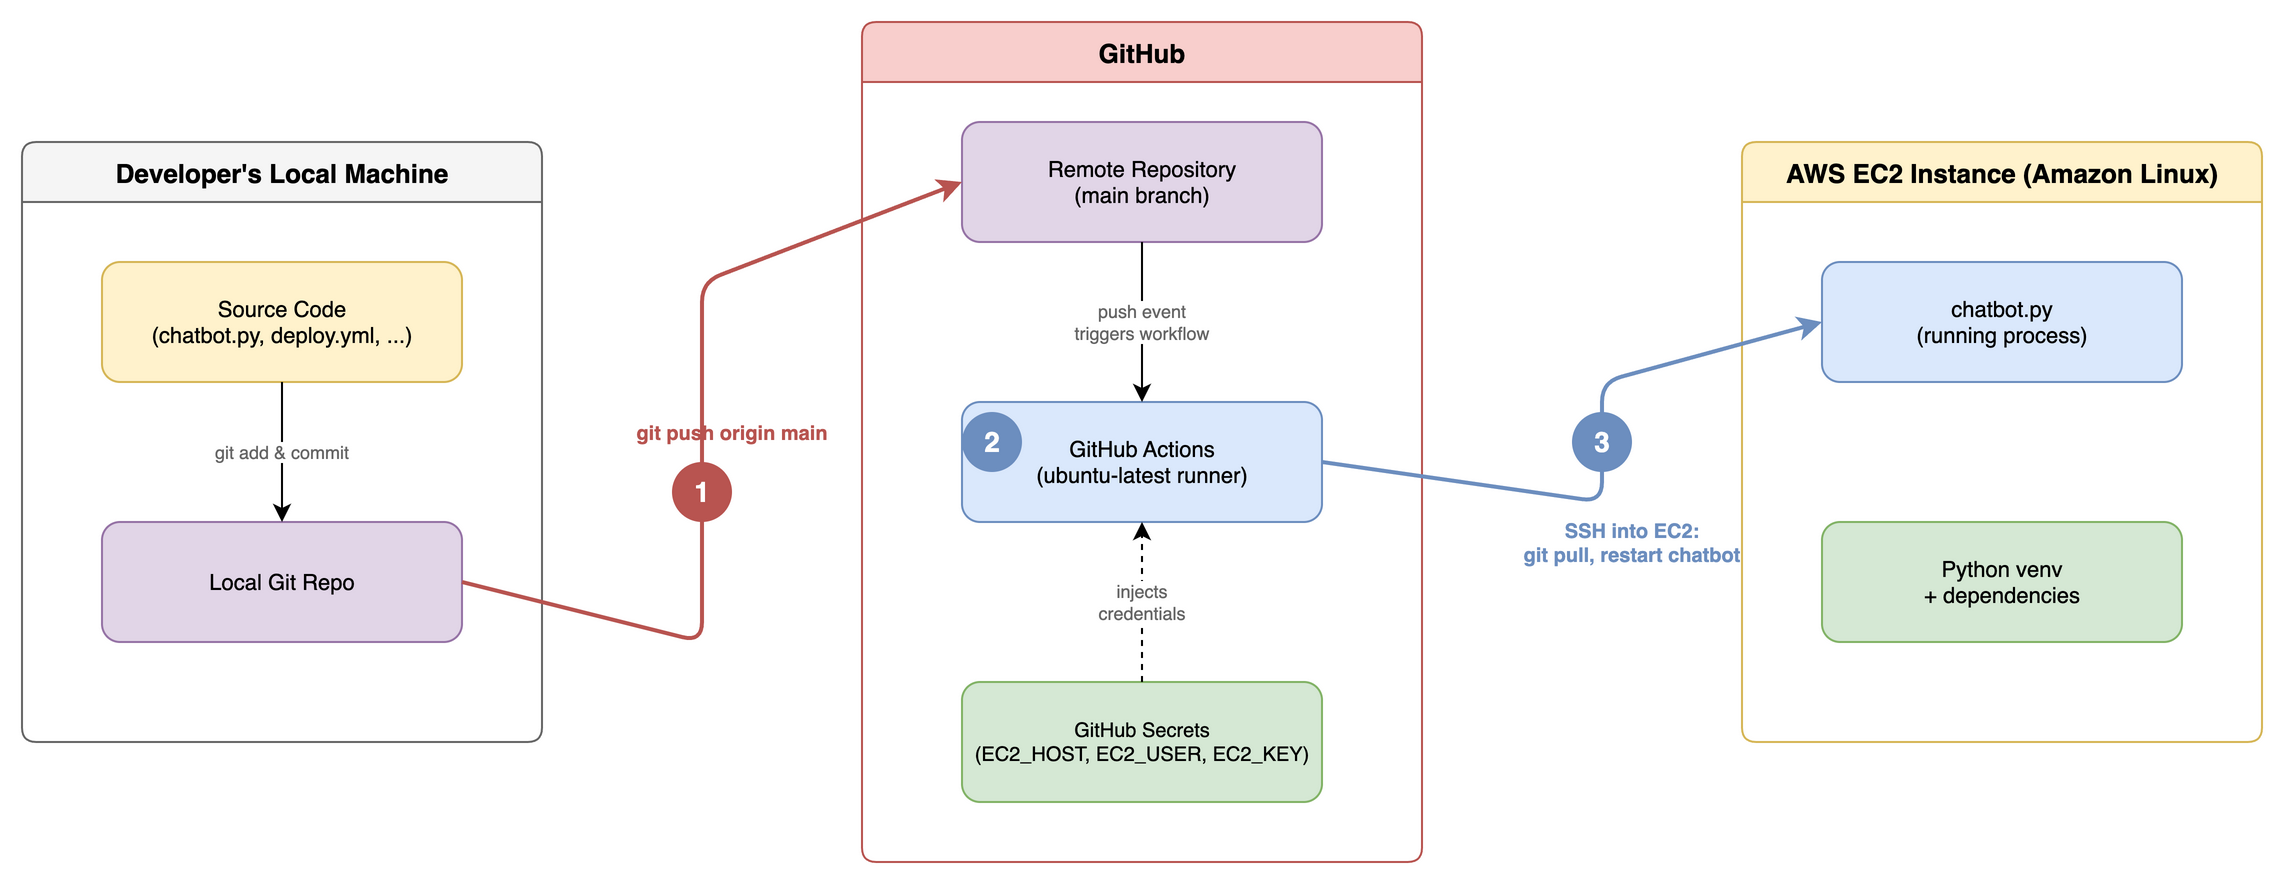
\includegraphics[width=0.95\linewidth]{lab5/cicd-flow.png}
  \caption{CI/CD data flow between the local repository, GitHub, and the AWS EC2 instance.}
  \label{fig:cicd}
\end{figure}

\subsection*{Q3: Why storing passwords in \texttt{config.ini} is insecure, and how GitHub Secrets improve security}

Storing sensitive credentials (such as API keys and access tokens) directly in \texttt{config.ini} is insecure for several reasons:

\begin{enumerate}
  \item \textbf{Version control exposure.}
    If \texttt{config.ini} is committed to a Git repository, the credentials become part of the repository history.
    Even if the file is later removed, the secrets remain recoverable from previous commits.
    If the repository is public, the credentials are exposed to anyone on the internet.

  \item \textbf{Plain-text storage.}
    The file stores secrets as plain text on disk.
    Anyone with access to the filesystem---whether through a compromised machine, a shared development environment, or a misconfigured server---can read the credentials directly.

  \item \textbf{No access control.}
    There is no built-in mechanism to restrict who can view or modify the contents of a plain configuration file.
    Any collaborator with repository access can read the secrets.
\end{enumerate}

GitHub Secrets address these issues by providing a secure, encrypted storage mechanism~\cite{github-actions-docs}:

\begin{itemize}
  \item \textbf{Encryption at rest.}
    Secrets are encrypted using Libsodium sealed boxes before being stored on GitHub's servers.
    They are only decrypted in memory on the runner during workflow execution and are never written to disk in plain text.

  \item \textbf{Masked in logs.}
    GitHub Actions automatically redacts secret values from workflow logs.
    Even if a command accidentally prints a secret, it appears as \texttt{***} in the log output.

  \item \textbf{Access control.}
    Only repository administrators can create or update secrets.
    Workflow files can reference secrets, but no user (including administrators) can view the secret values after they are saved.

  \item \textbf{Not stored in source code.}
    Secrets are managed outside the repository codebase, which eliminates the risk of accidental commits and exposure in version history.
\end{itemize}

\subsection*{Q4: GitHub Actions run screenshots}

Figure~\ref{fig:deploy-logs} shows the detailed logs of a successful GitHub Actions workflow run for the ``AWS EC2 Deploy'' workflow.
The run consists of several steps:

\begin{itemize}
  \item \textbf{Set up job:} The runner environment (\texttt{ubuntu-latest}) is initialized.
  \item \textbf{Checkout code:} The repository is cloned using \texttt{actions/checkout@v3}.
  \item \textbf{Setup SSH:} The SSH agent is started and the private key from \texttt{EC2\_KEY} is loaded via \texttt{webfactory/ssh-agent@v0.7.0}.
  \item \textbf{Deploy application:} The runner SSHs into the EC2 instance, pulls the latest code, and restarts the chatbot process. The logs show a successful connection to the Amazon Linux 2023 instance and a \texttt{git pull} completing with a fast-forward merge.
  \item \textbf{Post-job cleanup:} The SSH agent is stopped and temporary credentials are removed.
\end{itemize}

\begin{figure}[htbp]
  \centering
  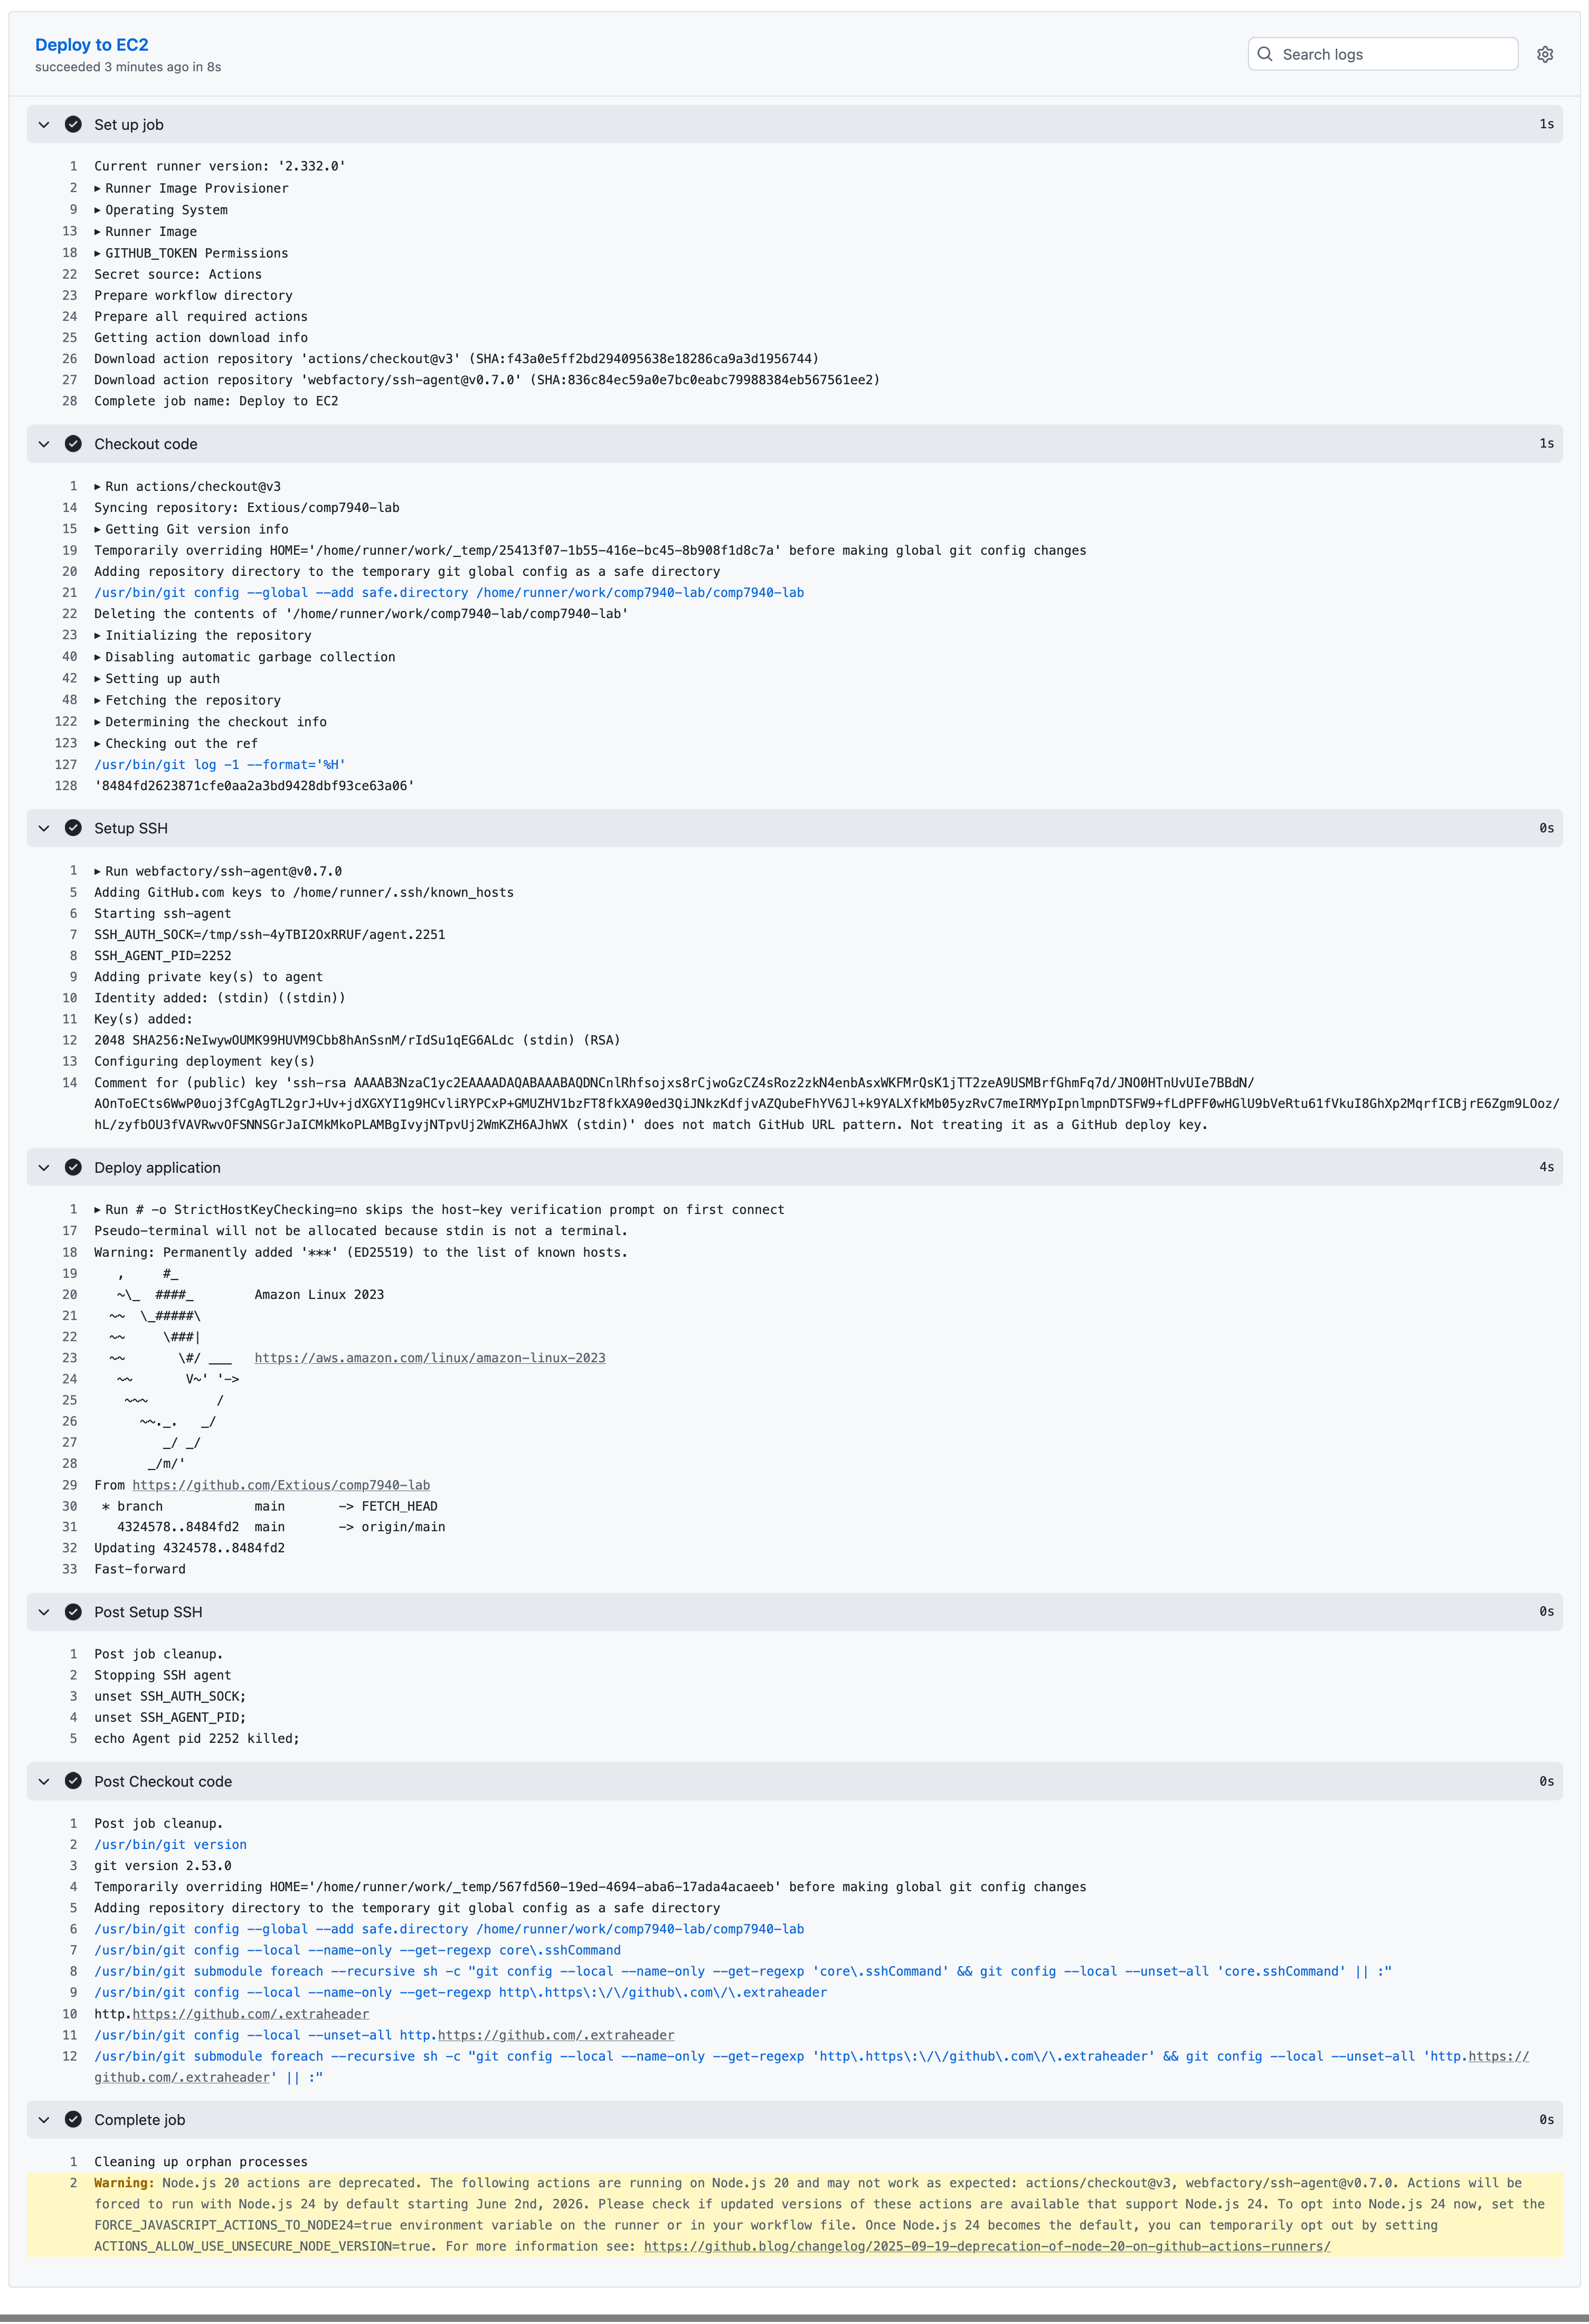
\includegraphics[width=0.85\linewidth]{lab5/deplog_logs.png}
  \caption{GitHub Actions workflow run logs for the ``AWS EC2 Deploy'' workflow, showing all steps completed successfully.}
  \label{fig:deploy-logs}
\end{figure}

Figure~\ref{fig:app-logs} shows the application logs (\texttt{app.log}) from the EC2 instance after deployment.
The chatbot initializes successfully: it loads configuration, connects to the Telegram API, registers the message handler, and begins polling for updates.
The repeated \texttt{getUpdates} HTTP requests confirm that the bot is running and actively listening for new messages.

\begin{figure}[htbp]
  \centering
  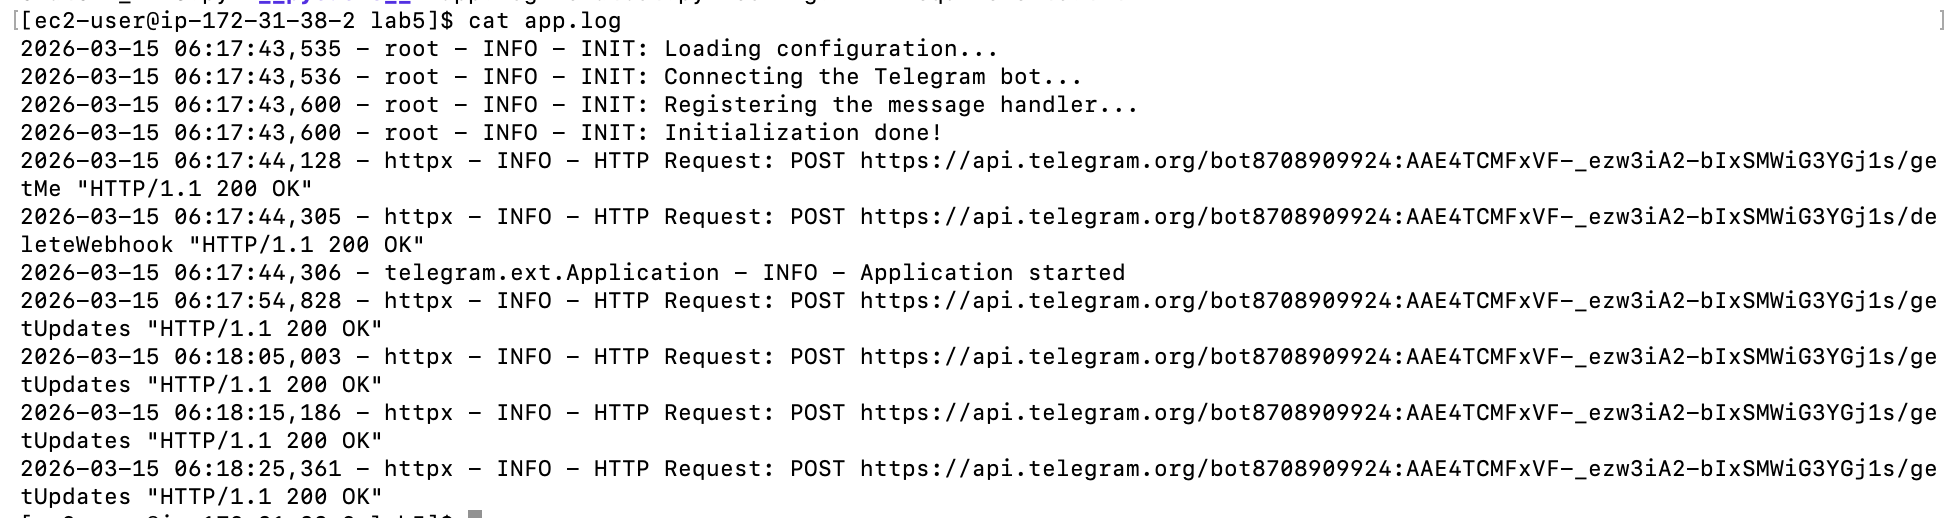
\includegraphics[width=0.95\linewidth]{lab5/app_logs.png}
  \caption{Application logs from the EC2 instance showing successful chatbot initialization and polling.}
  \label{fig:app-logs}
\end{figure}

\bibliographystyle{plain}
\bibliography{Lab5-25482351-ZHAOZhan}

\end{document}
